\pdfoutput=1
\documentclass[11pt]{amsart}
\usepackage{amsmath,amssymb,amsthm,mathtools}
\usepackage[margin=1.2in]{geometry}
\usepackage{graphicx,booktabs,adjustbox,tikz}
\usetikzlibrary{arrows.meta,positioning}
\usepackage{xcolor}
\usepackage[colorlinks=true,linkcolor=blue,citecolor=blue,urlcolor=blue]{hyperref}
\hypersetup{pdfauthor={Bernd Johannes Wuebben},
  pdftitle={Nonsimplicial local stability chambers of toric tangent bundles}}
\setlength{\emergencystretch}{2em}
\newtheorem{theorem}{Theorem}[section]
\newtheorem{proposition}[theorem]{Proposition}
\newtheorem{lemma}[theorem]{Lemma}
\newtheorem{corollary}[theorem]{Corollary}
\theoremstyle{definition}
\newtheorem{definition}[theorem]{Definition}
\newtheorem{example}[theorem]{Example}
\newtheorem{question}[theorem]{Question}
\theoremstyle{remark}
\newtheorem{remark}[theorem]{Remark}
\newcommand{\RR}{\mathbb R}
\newcommand{\CC}{\mathbb C}
\newcommand{\ZZ}{\mathbb Z}
\newcommand{\PP}{\mathbb P}
\newcommand{\cO}{\mathcal O}
\newcommand{\cC}{\mathcal C}
\newcommand{\rk}{\operatorname{rk}}
\newcommand{\im}{\operatorname{im}}
\newcommand{\Ext}{\operatorname{Ext}}
\newcommand{\Amp}{\operatorname{Amp}}
\newcommand{\cone}{\operatorname{cone}}
\newcommand{\spanR}{\operatorname{span}_{\RR}}
\newcommand{\spanC}{\operatorname{span}_{\CC}}
\newcommand{\one}{\mathbf1}
\title[Nonsimplicial tangent stability chambers]{Nonsimplicial local stability chambers\\of toric tangent bundles}
\author{Bernd Johannes Wuebben}
\subjclass[2020]{14M25 (primary); 14J60, 06A07, 52B20 (secondary)}
\keywords{toric variety, tangent bundle, slope stability, ample real divisor,
  partially ordered set, Harder--Narasimhan filtration}
\date{Original version: October 27, 2026\\This version: October 29, 2026}
\begin{document}
\begin{abstract}
We construct smooth projective toric varieties with nonsimplicial local
slope-stability chambers for their tangent bundles. In every even
dimension \(2k+2\ge4\), a fibre product of two projective-line bundles
over \((\PP^1)^{2k}\) admits an ample real class at which the tangent
bundle is strictly semistable. Near this class, the semistable locus
is analytically isomorphic to a pointed cone over
\(\Delta^1\times\Delta^{2k-1}\), times a line, where \(\Delta^j\)
denotes the \(j\)-simplex. The torus-invariant saturated subsheaves of
equal slope form the ideal lattice of the complete bipartite poset
with two minimal and \(2k\) maximal elements, and the stable line
factors realize every centered slope direction. These varieties are
weak Fano and not Fano. The fourfold has minimal dimension and Picard
rank among toric varieties with such a chamber and nearby stable
polarizations.
We also prove a local normal form at any ample real class where the
tangent bundle of a smooth projective toric variety is semistable.
It retains precisely the slope directions realized by polarizations,
requires no local-freeness assumption on equal-slope subsheaves, and
localizes every nearby Harder--Narasimhan filtration to their equality
lattice.
If the fan rays in each equal-slope subspace positively span that subspace,
every centered slope direction occurs. A semistable surface satisfies this condition although
one equal-slope quotient is not locally free.
\end{abstract}
\maketitle
\enlargethispage{5pt}


% ============================================================
% section_01_introduction.tex
% ============================================================
\section{Introduction}\label{sec01:intro}

Slope stability of a toric tangent bundle is determined by finitely many
linear inequalities in the numerical curve class of the polarization.
The inequalities are explicit, but their geometric occurrence is a
separate question. A cone constructed from an abstract partial order
need not occur as the local stability chamber of a tangent bundle.
We construct a family for which the entire equality lattice, the
accessible slope directions, and the tangent extension can all be
determined. Its smallest member has a square-cone chamber.

Throughout, projectivization parametrizes one-dimensional quotients.
For \(k\ge1\), put \(d=2k\), \(n=d+2\), and set
\begin{equation}\label{eq01:family}
 B=(\PP^1)^d,\quad L=\cO_B(1^k,-1^k),\quad
 X_k=\PP_B(\cO_B\oplus L)\times_B\PP_B(\cO_B\oplus L).
\end{equation}
Here \(1^k,-1^k\) means \(k\) entries equal to \(1\) followed by
\(k\) entries equal to \(-1\). Write \(h_j\) for the base hyperplane
classes, \(\xi_i\) for the two tautological classes, and
\[
 \ell=c_1(L),\qquad \eta_i=\xi_i-\ell/2,
 \qquad A=\eta_1+\eta_2,\qquad B_0=\sum_{j=1}^d h_j.
\]
The poset \(K_{2,d}\) has two minimal elements, \(d\) maximal elements,
and every minimal element is below every maximal element. An
\emph{order ideal} contains every predecessor of each of its elements.
An invariant saturated tangent subsheaf is an \emph{equality subsheaf}
at a semistable polarization if its slope equals that of the tangent
bundle. We include zero and the whole tangent bundle in their lattice.

For this family put \(C_1=2\eta_1\), \(C_2=2\eta_2\),
\(C_{j+2}=2h_j\), and \(D=\sum_pC_p=c_1(T_{X_k})\).
The centered line-factor degree vector is
\[
 z(H)=\bigl((C_p-D/n)H^{n-1}\bigr)_{p=1}^n,
 \qquad \sum_p z_p(H)=0.
\]
Thus its coordinates are the line-factor slopes after subtracting
their mean. Saying that every such direction is realized locally
means that the differential of \(H\mapsto z(H)\) is onto the
zero-sum hyperplane.

\begin{theorem}\label{thm01:family}
For every \(k\ge1\), there is a unique \(r_k>1\) such that the line
bundles with first Chern classes
\(2\eta_1,2\eta_2,2h_1,\ldots,2h_d\) have equal slope at
\(H_0=A+r_kB_0\). This class is ample, and \(T_{X_k}\) is strictly
semistable there. The following assertions hold.
\begin{enumerate}
\item The equality subsheaves form the ideal lattice of \(K_{2,d}\).
Adjoining one poset element to an ideal increases the rank of its
corresponding subsheaf by one. The differential of \(H\mapsto z(H)\)
at \(H_0\) is surjective onto the zero-sum hyperplane.
\item In real analytic coordinates centered at \(H_0\), the local
semistable set is the germ of
\begin{equation}\label{eq01:cone}
 \left\{z\in\RR^{d+2}:\ \sum_pz_p=0,\quad
 z_1,z_2\le0,\quad z_3,\ldots,z_{d+2}\ge0\right\}\times\RR.
\end{equation}
The stable set is obtained by making all displayed sign inequalities
strict. The pointed cone has dimension \(d+1\), \(2d\) rays,
\(d+2\) facets, and a section \(\Delta^1\times\Delta^{d-1}\).
It is not simplicial.
\item For \(\pi:X_k\to B\), the actual tangent sequence is
\begin{equation}\label{eq01:extension}
 0\longrightarrow R_1\oplus R_2\longrightarrow T_{X_k}
 \longrightarrow\bigoplus_{j=1}^d Q_j\longrightarrow0,
 \qquad
 R_i=\cO_{X_k}(2\xi_i)\otimes\pi^*L^{-1},\quad
 Q_j=\pi^*\cO_B(2h_j).
\end{equation}
These are pairwise nonisomorphic stable line factors at \(H_0\).
All \(2d\) components in \(\Ext^1(Q_j,R_i)\) are nonzero.
Every specified saturated equivariant equality subsheaf is a relative
tangent bundle of a smooth projection.
\end{enumerate}
The variety \(X_k\) is weak Fano and is not Fano. For \(k=1\),
\(r_1=(3+\sqrt{21})/6\), and \(\dim X_1=\rho(X_1)=4\).
Both dimensions are minimal for a nonsimplicial pointed chamber at a
strictly semistable class with a nearby stable locus.
\end{theorem}

Sections~\ref{sec05:family}--\ref{sec07:extension} prove this theorem
from the fan, intersections, and tangent transitions. No analytic
existence or spectral comparison is used to establish the geometry.

We also prove a local normal form without assuming that equality
subsheaves are subbundles. The equality lattice determines a poset
\(P\), positive integer block ranks \(r_p\), and block divisor
classes \(C_p\). For \(D=c_1(T_X)\), define the centered slope map
\[
 \mathcal A(\alpha)_p=(C_p-r_pD/n)\cdot\alpha,
 \qquad L_{\rm acc}=\im\mathcal A\subset
 Z=\{z\in\RR^P:\sum_pz_p=0\}.
\]
Theorem~\ref{thm03:normal} identifies the local semistable germ with
\((\cC(P)\cap L_{\rm acc})\times\RR^{\rho-\dim L_{\rm acc}}\),
where \(\cC(P)\) is defined by nonpositive sums on order ideals.
The accessible image is essential: different sections of the same
poset cone can have different faces or no strict stable direction.
Proposition~\ref{prop04:character} gives a character criterion for
this failure for any fixed toric equality data.

Nonsimpliciality distinguishes differentiable chamber germs, rather
than their ordinary topology. Under strict feasibility, the semistable
and stable germs are ambiently bi-Lipschitz equivalent to a closed and
open halfspace pair (Proposition~\ref{prop04:topology}). The equality
lattice also controls more than the stable set: after a single shrink,
every nearby ordinary Harder--Narasimhan filtration uses only its
original equality subsheaves. Theorem~\ref{thm08:hn} identifies the
region of each filtration flag and gives its product form. For
\(X_k\) all flags occur; there are \(6F(2k)\), where \(F\) is the
ordered Bell number. For the fourfold there are eighteen flags, thirteen
of full dimension in the three-dimensional centered slope space.

\subsection*{Proof strategy}
The ray set of our family is the union of two lattice bases. At the
equal-slope class every ray divisor has the same degree, so the two
basis rank bounds prove semistability and classify all equality
cases at once. To produce that class inside the ample cone, we compute
the volume along a symmetric line. Its derivative gives a scalar
equal-slope equation; a normalized ample affine line and the strict
real Hodge inequality prove a unique simple root. Independent block
divisor classes then give every centered slope direction.

For the general local model, positivity makes the tight ray sets a
distributive lattice. The real numerical Hodge isomorphism turns
ample powers into local coordinates, leaving exactly the ideal
inequalities restricted to the actual slope image. Finally, we apply
the finite ray-span argument simultaneously to every equality
quotient. One common neighborhood excludes all initially strict
competitors, so the HN problem becomes maximal-average selection
on the original ideal lattice. Semistability of its successive
intervals gives the stated product regions.

\subsection*{Relation to earlier work}
Klyachko's filtrations describe equivariant bundles and the distinction
between invariant saturated subsheaves and genuine subbundles
\cite{klyachko1990}; see also \cite[Proposition~4.1.1]{khandasgupta2019}.
Hering--Nill--S\"u\ss give the finite tangent slope test and explicitly
describe its curve-class inequalities
\cite[Proposition~1.2, Remark~2.6, and \S5]{heringnillsuess2022}.
Neumann's and Pang's work already supplies ordinary real-class
Harder--Narasimhan theory, torus invariance, polyhedrality, and
successive quotient computations
\cite[\S3.3]{neumann2009}\cite[\S\S1.3,2.1--2.2]{pang2015}.
Our local equality-interval description and its products refine these
results near a fixed semistable class; a general HN algorithm or
curve-class polyhedrality is not a new assertion here.

The equality-poset construction and a chamber normal form under a
cone-wise equality-subbundle hypothesis appear in
\cite{wuebben2026toricchambers}. We retain that construction, remove the
hypothesis from the numerical normal form by keeping the actual slope
image, and prove the realizability theorem above. The root-cone ray
and simpliciality criteria are those of
Boussicault--F\'eray--Lascoux--Reiner
\cite[\S5]{boussicaultferaylascouxreiner2012}, with the edge sign
reversed. Our family realizes their nonsimplicial cone by actual toric
tangent bundles.

This geometry is the independent algebraic input to a three-paper
programme on stability and loss of analytic rigidity. The companion
spectral work treats actual Hermitian--Einstein metrics on two-step
extensions; the subsequent quantitative work adds inverse, response,
and flow estimates and states the integrated theorem on the same
\(T_{X_k}\). Section~\ref{sec09:fourfold} specifies the slope
normalization and parameter chart supplied here. The harmonic metric
coefficients required by that analysis are additional data.

% ============================================================
% section_02_equality.tex
% ============================================================
\section{Real polarizations and the equality lattice}\label{sec02:equality}

Let \(X=X_\Sigma\) be a smooth projective toric variety of dimension
\(n\ge2\), with lattice \(N\), dual lattice \(M\), primitive ray
vectors \(v_\rho\), and invariant prime divisors \(D_\rho\).
We use ordinary intersection degrees
\[
 \deg_H\mathcal F=c_1(\mathcal F)H^{n-1},\qquad
 \mu_H(\mathcal F)=\deg_H\mathcal F/\rk\mathcal F
\]
for a nonzero torsion-free sheaf and an ample real divisor class
\(H\in N^1(X)_\RR\). Stability always means stability against all
coherent subsheaves of smaller positive rank. It suffices to test
saturated subsheaves, whose quotients are torsion free.

The torus trivialization of \(T_X\) identifies its equivariant generic
fibre with \(N_\CC\). For a complex subspace \(V\subset N_\CC\),
let \(\mathcal F_V\) be the unique saturated equivariant subsheaf
with generic fibre \(V\). The tangent filtrations give
\begin{equation}\label{eq02:degree}
 \rk\mathcal F_V=\dim V,\qquad
 c_1(\mathcal F_V)=\sum_{v_\rho\in V}D_\rho.
\end{equation}
For example, at the divisor of a ray the tangent filtration has the
single intermediate line \(\CC v_\rho\). Its induced filtration on
\(V\) contributes one to the first Chern coefficient precisely when
that line lies in \(V\). This proves \eqref{eq02:degree} from the
codimension-one filtrations; see
\cite[\S2]{heringnillsuess2022}\cite[Theorem~2.1.8]{pang2015}.
Neither saturation nor this calculation asserts local freeness.

\begin{lemma}\label{lem02:realtest}
For an ample real \(H\), ordinary slope (semi)stability of \(T_X\)
is equivalent to
\begin{equation}\label{eq02:test}
 \frac{\sum_{v_\rho\in V}D_\rho H^{n-1}}{\dim V}
 \ \mathrel{(<)}\le\ \frac{\sum_\rho D_\rho H^{n-1}}n
 \qquad(0\ne V\subsetneq N_\CC).
\end{equation}
Only spans of subsets of ray vectors need be tested.
\end{lemma}

\begin{proof}
For an integral ample class this is the tangent criterion of
\cite[Proposition~1.2 and Remark~2.6]{heringnillsuess2022}.
The reduction to equivariant subsheaves also works at a real class,
including equality. Choose an auxiliary integral torus-linearized
ample line bundle to form a projective Quot scheme. The closure of
the torus orbit of a quotient \(T_X\twoheadrightarrow\mathcal Q\)
contains a torus-fixed quotient: one can successively take limits
along one-parameter subgroups of the torus in a projective embedding.
In this connected flat family, the rank and numerical first Chern
class of the quotient, and hence of its kernel, are constant.
Indeed the determinant of the flat family defines a family of line
bundles on \(X\). Since \(\operatorname{Pic}(X)\) is discrete,
its class is constant on the connected orbit closure. This fixes
the full numerical first Chern class, not just its degree against
the auxiliary polarization.
Saturating the fixed kernel makes it equivariant and adds an
effective divisorial class to its first Chern class. Such a class
has nonnegative degree against \(H^{n-1}\). Thus any ordinary
subsheaf violating either stability test gives an equivariant one
with at least its real slope. Equation~\eqref{eq02:degree} now gives
\eqref{eq02:test}.

Every \(D_\rho H^{n-1}\) is positive. If \(V\) contains a ray,
its contained-ray span \(W\) has the same numerator as \(V\) and
no larger dimension; its slope is at least that of \(V\).
If it contains no ray, its slope is zero, strictly smaller than
\(\mu_H(T_X)>0\). This proves the finite reduction.
\end{proof}

Fix henceforth an ample real \(H_0\) at which \(T_X\) is semistable.
Write
\begin{equation}\label{eq02:weights}
 \alpha_0=H_0^{n-1},\quad D=\sum_\rho D_\rho,
 \quad w_\rho=D_\rho\alpha_0>0,\quad
 \tau=D\alpha_0/n>0.
\end{equation}
A subspace \(V\) is \emph{tight} if
\(\sum_{v_\rho\in V}w_\rho=\tau\dim V\); zero and \(N_\CC\)
are tight. A \emph{ray flat} is the full set of rays in a subspace
spanned by rays. Tight subspaces are ray-spanned by the proof above,
since reducing the dimension would otherwise violate semistability.

\begin{proposition}\label{prop02:lattice}
The ray sets of the tight subspaces form a finite distributive lattice
under union and intersection. There is a finite poset \(P\) of ray
blocks such that these sets are exactly its order ideals. There are
positive integers \(r_p\) and divisor classes
\(C_p=\sum_{\rho\text{ in block }p}D_\rho\) satisfying
\begin{equation}\label{eq02:ranks}
 \sum_{p\in P}r_p=n,\qquad C_p\alpha_0=\tau r_p.
\end{equation}
For an ideal \(I\), its tight subspace \(V_I\) and equality subsheaf
\(\mathcal F_I=\mathcal F_{V_I}\) have
\(\dim V_I=r(I):=\sum_{p\in I}r_p\) and
\(c_1(\mathcal F_I)=C_I:=\sum_{p\in I}C_p\).
\end{proposition}

\begin{proof}
Put \(w(V)=\sum_{v_\rho\in V}w_\rho\). For tight \(V,W\),
\[
 w(V)+w(W)\le w(V+W)+w(V\cap W)
 \le\tau\bigl(\dim(V+W)+\dim(V\cap W)\bigr)
 =w(V)+w(W).
\]
All inequalities are equalities. Positivity of the ray weights shows
that \(V+W\) contains no ray outside the union of the two ray sets.
The intersection ray set is already their set intersection.
Both subspaces are tight and ray-spanned. Their ray sets therefore
determine them, proving the distributive-lattice assertion.

Declare two rays equivalent when they belong to exactly the same
tight sets, and call the equivalence classes blocks. For a block
\(q\), let \(J_q\) be the intersection of all tight sets containing
it. Define \(p\le q\) if block \(p\) lies in \(J_q\).
This is a partial order: antisymmetry is precisely the block
equivalence, and transitivity follows because \(q\subset J_r\)
implies \(J_q\subset J_r\). By definition,
\(J_q=\bigcup_{p\le q}p\). Each tight set is an ideal, while every ideal is the
union of its \(J_q\); these unions are tight. Thus we have exactly
the asserted ideal lattice.

Both \(J_p\) and \(J_p\setminus\{p\}\) are ideals. Their rank
difference is the positive integer
\[
 r_p=\dim V_{J_p}-\dim V_{J_p\setminus\{p\}}
     =\frac{\sum_{\rho\text{ in block }p}w_\rho}{\tau}.
\]
Telescoping along a linear extension of any ideal proves all the
rank and Chern-class formulas, including \eqref{eq02:ranks}.
\end{proof}

We call \(P\) the \emph{equality poset}. This is the poset whose ideal
lattice is the lattice of invariant saturated equality subsheaves;
it does not specify a locally free associated graded bundle or its
extension classes. The construction agrees with
\cite[\S3]{wuebben2026toricchambers} and uses no additional
cone-wise subbundle hypothesis.

% ============================================================
% section_03_normal.tex
% ============================================================
\section{The accessible local normal form}\label{sec03:normal}

For a finite poset \(P\), put
\begin{equation}\label{eq03:root}
 Z=\{z\in\RR^P:\sum_pz_p=0\},\qquad
 \cC(P)=\{z\in Z:\ z(I):=\sum_{p\in I}z_p\le0
                       \text{ for every order ideal }I\}.
\end{equation}
Write \(\cC^{\rm str}(P)\) for the locus where every proper nonempty
ideal inequality is strict. For a one-element poset it is \(\{0\}\).
The cone is the upward poset root cone: if \(p\lessdot q\) is a
cover, let \(u_{pq}=e_q-e_p\). Our sign is opposite to that of
\cite[\S5]{boussicaultferaylascouxreiner2012}.
Here \(e_p\) denotes the standard coordinate vector of \(\RR^P\),
independently of the lattice basis used later to describe a toric fan.

\begin{lemma}\label{lem03:root}
We have \(\cC(P)=\cone\{u_{pq}:p\lessdot q\}\). Its span has
dimension \(|P|-c(P)\), where \(c(P)\) is the number of connected
components of the undirected Hasse graph. Its extreme rays are exactly
the cover vectors, and it is simplicial precisely when that graph is
a forest. If \(P\) is connected, \(\cC^{\rm str}(P)\) is its
interior in \(Z\), and consists of positive combinations of all
cover vectors. If \(P\) is disconnected with at least two elements,
the strict locus is empty.
\end{lemma}

\begin{proof}
An upward edge has ideal sum either zero or minus one, giving the
first inclusion. A functional nonnegative on all edge vectors is an
order-preserving potential, modulo a constant. Express it as a
constant plus a nonnegative combination of upper-level-set
indicators. Their complements are ideals, so it is nonnegative on
\(\cC(P)\). Separation from the closed finitely generated edge cone
gives the reverse inclusion. Incidence rank gives the dimension.
The extreme-ray and forest assertions are the root-cone statements
of \cite[Proposition~5.1(i) and Corollary~5.3]{boussicaultferaylascouxreiner2012}.

For connected \(P\), the sum of all cover vectors has a strictly
negative sum on every proper nonempty ideal: such an ideal has an
edge leaving it. Conversely, from any strict point one may subtract
a sufficiently small positive multiple of this vector and remain in
the cone. This gives a representation with every edge coefficient
positive and proves the interior assertion. In the disconnected case
a component and its complement are proper ideals; both sums cannot
be negative. The relative interior still has positive edge
representations in the component-zero-sum span, but it is not the
strict stable locus.
\end{proof}

Return to the equality data of Section~\ref{sec02:equality}. The
numerical curve space \(N_1(X)_\RR\) is dual to \(N^1(X)_\RR\).
Both have dimension \(\rho\). Define
\begin{equation}\label{eq03:accessible}
 K_p=C_p-\frac{r_p}{n}D,\qquad
 \mathcal A:N_1(X)_\RR\longrightarrow Z,\quad
 \mathcal A(\alpha)_p=K_p\alpha,
 \qquad L_{\rm acc}=\im\mathcal A,\quad a=\dim L_{\rm acc}.
\end{equation}
The name \emph{accessible slope space} means precisely this linear
image, not an independently prescribed subspace of \(Z\).
By \eqref{eq02:ranks}, \(\mathcal A(\alpha_0)=0\).

\begin{theorem}\label{thm03:normal}
Let \(X\) be smooth projective toric, \(n\ge2\), and let \(T_X\)
be semistable at an interior ample real class \(H_0\). In real
analytic coordinates centered at \(H_0\), the pair of local
semistable and stable sets is the germ of
\begin{equation}\label{eq03:normal}
 \left(
  (\cC(P)\cap L_{\rm acc})\times\RR^{\rho-a},\quad
  (\cC^{\rm str}(P)\cap L_{\rm acc})\times\RR^{\rho-a}
 \right).
\end{equation}
In particular, stable ample classes approach \(H_0\) if and only if
\(L_{\rm acc}\) meets \(\cC^{\rm str}(P)\). No local-freeness
assumption on \(\mathcal F_I\) is needed.
\end{theorem}

\begin{proof}
The Hodge--Riemann bilinear relations for the Kähler class \(H_0\),
restricted to \(N^1(X)_\RR\), give the real numerical Hodge index
theorem. Thus
\(E\mapsto H_0^{n-2}E\) is an isomorphism
\(N^1(X)_\RR\to N_1(X)_\RR\)
\cite[Theorem~6.4 and Corollary~6.5]{grebrosstoma2016}.
Consequently the derivative of the polynomial power map
\(\Psi(H)=H^{n-1}\) is the isomorphism
\((n-1)H_0^{n-2}(-)\). The analytic inverse-function theorem gives
an open neighborhood of \(\alpha_0\) consisting entirely of powers
of actual ample real classes.

There are finitely many ray-flat tests. Those strict at \(H_0\)
remain strict on a common neighborhood. The remaining tests are
exactly the tight ideals, and their centered degrees are
\[
 (C_I-r(I)D/n)\alpha=\sum_{p\in I}\mathcal A(\alpha)_p.
\]
Thus the semistable and stable inequalities are exactly those of
\eqref{eq03:root} and its strict locus there.

Choose a linear right inverse \(J:L_{\rm acc}\to N_1(X)_\RR\)
of \(\mathcal A\). The explicit coordinates are
\begin{equation}\label{eq03:coordinates}
 z=\mathcal A(\alpha-\alpha_0),\qquad
 t=\alpha-\alpha_0-Jz\in\ker\mathcal A,
 \qquad\alpha=\alpha_0+Jz+t.
\end{equation}
These prove \eqref{eq03:normal}. A strict \(z\) lifts along
\(\alpha_0+\varepsilon Jz\) for every sufficiently small
\(\varepsilon>0\); its inverse power is ample, preserves all the
initially strict tests, and makes the remaining tests strict.
The converse follows by applying \(\mathcal A\).
\end{proof}

The cone-wise hypothesis called condition~(15) in
\cite{wuebben2026toricchambers} requires every tight subspace \(V\)
to contain \(\dim V\) ray generators of each maximal cone. It is
a genuine additional geometric hypothesis: the simultaneous bases
then make the specified equality subsheaves subbundles. The preceding
theorem removes it from the numerical local model by retaining
\(L_{\rm acc}\); it does not remove it from a local-freeness claim.
In particular, the classes \(C_p\) in general are divisor sums,
not asserted Chern classes of stable vector-bundle factors.

\begin{example}\label{ex03:section}
Sections can change the cone even for a tree poset. A four-edge star
with upward coordinates \(a_1,\ldots,a_4\) has cone
\(\RR_{\ge0}^4\). Its section
\(a_1+a_2=a_3+a_4\) is a three-dimensional cone with four rays
generated by \(e_1+e_3,e_1+e_4,e_2+e_3,e_2+e_4\), where these
are the coordinate vectors of the nonnegative orthant. No toric realization
of this section is asserted. Also, for the three-element star
\(0<1,0<2\), the line \(\spanR(0,1,-1)\subset Z\) misses the
strict cone although the poset is connected. These examples explain
why a Hasse-cycle criterion for the full cone is not a criterion for
an arbitrary accessible section.
\end{example}

% ============================================================
% section_04_topology.tex
% ============================================================
\section{Feasibility, topology, and dimension bounds}\label{sec04:topology}

The image in \eqref{eq03:accessible} permits a precise alternative
between an accessible stable direction and an order-preserving
numerical relation. Write \(M_\RR=M\otimes\RR\).

\begin{proposition}\label{prop04:character}
Suppose that \(P\) is connected and \(|P|\ge2\). Then
\(L_{\rm acc}\cap\cC^{\rm str}(P)=\varnothing\) if and only if
there exist numbers \(a_p\), not all zero, such that
\begin{equation}\label{eq04:character}
 p\le q\ \Longrightarrow\ a_p\le a_q,\qquad
 \sum_pr_pa_p=0,\qquad \sum_pa_pC_p=0\quad\hbox{in }N^1(X)_\RR.
\end{equation}
Equivalently there is a nonzero \(m\in M_\RR\) whose values
\(\langle m,v_\rho\rangle=a_p\) are constant on each ray block
and order-preserving on \(P\).
\end{proposition}

\begin{proof}
The connected root cone is full-dimensional in \(Z\). Separation of
its interior from a subspace is equivalent to a nonzero dual class
\([a]\in\cC(P)^*\cap L_{\rm acc}^{\perp}\), where potentials
are considered modulo constants. Pairing with each upward cover
vector says exactly that \(a\) is order-preserving.
Orthogonality to \(\im\mathcal A\) says
\[
 \sum_pa_pC_p-\frac{\sum_pr_pa_p}{n}D=0.
\]
Subtract the rank-weighted mean from every \(a_p\). This gives
\eqref{eq04:character} and preserves its nonzero class and order.
Conversely those conditions give the separating dual class.

For a smooth complete toric variety the kernel of the real invariant
divisor map to \(N^1(X)_\RR\) consists of principal real divisors:
\(m\mapsto\sum_\rho\langle m,v_\rho\rangle D_\rho\).
Here the divisor class group equals the Picard group, and numerical
and real linear equivalence agree, so this is also the numerical
kernel. Applying this sequence to \(\sum_pa_pC_p\) gives the
character formulation. Pairing that relation with \(\alpha_0\)
already forces the rank centering in \eqref{eq04:character}.
The rays span \(N_\RR\), so a nonzero coefficient vector gives
a nonzero character and conversely.
\end{proof}

This decides feasibility for a specified pair of toric equality data.
It neither asserts that such a nonzero obstruction occurs on a toric
variety nor proves universal accessibility. Disconnected posets must
be treated separately: their strict locus is empty even if the block
classes are independent.

\subsection*{Positive spanning and local freeness}

The cone-wise subbundle condition is stronger than what is needed for
full numerical access. The following condition uses only the rays in
each tight subspace, rather than their occurrence in each maximal cone.

\begin{proposition}\label{prop04:positive}
Suppose that, for every tight subspace $V$, the fan rays contained in
$V_\RR$ positively span $V_\RR$. Then the classes $C_p$ are linearly
independent in $N^1(X)_\RR$, so $L_{\rm acc}=Z$. Consequently stable
ample classes approach $H_0$ if and only if $X$ is not a nontrivial
toric product. This condition does not assert local freeness of
equal-slope quotients.
\end{proposition}

\begin{proof}
Write a numerical relation $\sum_p a_pC_p=0$ as a principal real
divisor. Thus some $m\in M_\RR$ takes the value $a_p$ on every ray
of block $p$. Choose a linear extension $p_1,\ldots,p_s$ of $P$.
Each initial ideal $I_j$ is tight. Its positive-spanning hypothesis
gives a relation
\[
 \sum_{\rho\in I_j}b_\rho v_\rho=0,\qquad b_\rho>0.
\]
Indeed express the negative of each ray as a nonnegative combination
of the contained rays and add these relations. If the coefficients
$a_{p_i}$ vanish for $i<j$, pairing with $m$ leaves
$a_{p_j}\sum_{\rho\in p_j}b_\rho=0$. Induction proves that every
$a_p$ vanishes. The centered classes therefore have rank $s-1$,
and Theorem~\ref{thm03:normal} gives the full cone.

By Lemma~\ref{lem03:root}, its strict locus is nonempty exactly when
$P$ is connected. If $P$ is disconnected, complementary unions of
components are tight ideals whose ray spans are complementary.
A maximal-cone lattice basis splits the lattice into these summands;
completeness then supplies every combination of component cones.
Thus $X$ is a toric product. Conversely, a toric product splits $T_X$
into nonzero summands. Semistability forces both summands to have the
common slope, giving complementary tight ideals and a disconnected
$P$. This also proves the final equivalence.
\end{proof}

The independence argument is the positive-relation argument of
\cite{wuebben2026toricchambers}, with its sufficient hypothesis
separated from the local-freeness condition. The latter implies
positive spanning because the cones contained in a tight subspace
form a complete subfan. The converse fails even for a semistable
tangent bundle on a toric surface.

\begin{example}\label{ex04:singularquotient}
Let $X$ have rays
\[
 v=(1,0),\quad -v=(-1,0),\quad b=(0,1),\quad
 b'=(1,-1),\quad w=(1,1),
\]
and cyclic maximal cones
$(v,w),(w,b),(b,-v),(-v,b'),(b',v)$. Each is unimodular.
This is the blowup $\pi:X\to\mathbb F_1$ of the fixed point of
$(v,b)$. Let $S$ be the negative section, $f$ a fibre and $E$ the
exceptional divisor. Set
\[
 H_t=\pi^*(4S+(7+t)f)-2E.
\]
In the displayed ray order its divisor coefficients can be taken to
be $(4,0,0,7+t,2)$. The moment polygon is
\[
 -4\le x\le0,\qquad 0\le y\le x+7+t,\qquad x+y\ge-2.
\]
For $t>-1$ its five vertices are
$(-4,2),(-2,0),(0,0),(0,7+t),(-4,3+t)$, with precisely the stated
normal cones. Its invariant divisor degrees are
\begin{equation}\label{eq04:surfacedegrees}
 (D_vH_t,D_{-v}H_t,D_bH_t,D_{b'}H_t,D_wH_t)
       =(1+t,7+t,2,4,2).
\end{equation}
Thus $H_t$ is ample exactly for $t>-1$. The line $\RR v$, which
is the original fibre tangent direction, contains two rays and has
degree $8+2t$, whereas the other ray lines have degrees $2,4,2$.
Since $\mu_{H_t}(T_X)=8+t$, these are all the proper ray-flat tests:
$T_X$ is stable for $-1<t<0$, strictly semistable at $t=0$, and
unstable for $t>0$.

At $t=0$ the only proper tight subspace is $\RR v$. Its two rays
positively span it, but the cone $(w,b)$ contains no ray of that line.
Condition~(15) therefore fails. In its smooth affine chart $v=w-b$,
and the induced tangent line has inclusion generated by
$x\partial_x-y\partial_y$. The exact sequence is
\[
 0\longrightarrow\cO\xrightarrow{\,1\mapsto(x,-y)\,}\cO^2
 \xrightarrow{\,(a,b)\mapsto ya+xb\,}(x,y)\longrightarrow0.
\]
The ideal $(x,y)$ is torsion-free but not locally free at the origin.
Globally the equality subsheaf is
$\cO_X(\pi^*(2S+f)-E)$ and its quotient is $\mathcal I_p(2f)$
for this fixed point $p$. Thus the subsheaf is a line bundle but its
inclusion is not a vector-subbundle inclusion. Full numerical access
cannot replace the regularity assumptions in an HE application.
Existence of stable polarizations here is also a consequence of the
toric surface classification in \cite[Theorem~1.3]{heringnillsuess2022};
the example separates the geometric hypotheses, rather than providing
a new surface existence theorem.
\end{example}

\begin{proposition}\label{prop04:topology}
Assume that \(H_0\) is strictly semistable and that nearby stable
classes exist. Put \(K=\cC(P)\cap L_{\rm acc}\) and
\(f=\rho-\dim L_{\rm acc}\). Then \(K\) is a full-dimensional
pointed cone in \(L_{\rm acc}\), and its interior is
\(\cC^{\rm str}(P)\cap L_{\rm acc}\). The pair
\((K\times\RR^f,\operatorname{int}K\times\RR^f)\) is ambiently
and positively homogeneously bi-Lipschitz homeomorphic to a closed
and open halfspace pair in \(\RR^\rho\). Its spherical semistable
link is a closed \((\rho-1)\)-ball, with stable part its interior.
\end{proposition}

\begin{proof}
Choose a strict \(v\in L_{\rm acc}\). For each proper nonempty
ideal put \(\ell_I(z)=-z(I)\), so \(\ell_I(v)>0\).
These finitely many functionals cut out \(K\). Strict inequalities
are exactly its interior; adding \(\varepsilon v\) to any point
proves that this interior has closure \(K\). The full root cone is
pointed: a strictly increasing potential has positive value on every
nonzero positive combination of upward cover vectors. Its section is
pointed as well. The poset is connected by Lemma~\ref{lem03:root}.

Write the ambient vector as \(y+tv\), where \(y\) ranges over a
complement to \(\RR v\) in \(L_{\rm acc}\), together with all
free coordinates. The latter are ignored by every \(\ell_I\).
Then
\[
 y+tv\in K\times\RR^f
 \quad\Longleftrightarrow\quad
 t\ge\phi(y),\qquad
 \phi(y)=\max_I\frac{-\ell_I(y)}{\ell_I(v)}.
\]
The finite maximum \(\phi\) is Lipschitz and positively homogeneous.
The ambient map \((y,t)\mapsto(y,t-\phi(y))\) and its inverse
are Lipschitz and carry strict epigraphs to open halfspaces. Radial
normalization gives the link statement. Free directions lie on the
boundary. Composing with the analytic coordinates of
Theorem~\ref{thm03:normal} gives the local toric assertion.
\end{proof}

A differentiable equivalence preserves more information. Its derivative
at the vertex is an invertible linear map taking tangent cones to
tangent cones. It therefore preserves lineality and the face lattice
of the pointed quotient. A nonsimplicial pointed cone cannot become
an orthant under such an equivalence, even though Proposition
\ref{prop04:topology} removes its corners topologically. Here and below
the lineality is the largest vector subspace contained in the cone.

\begin{proposition}\label{prop04:dimension}
Under the hypotheses of Proposition~\ref{prop04:topology}, a
nonsimplicial pointed chamber requires \(n\ge4\) and \(\rho\ge4\).
If \(n=4\), then \(|P|=4\), every \(r_p=1\),
\(\dim L_{\rm acc}=3\), and \(L_{\rm acc}=Z\). Its Hasse graph
is a four-cycle, with the poset either a diamond or \(K_{2,2}\).
In either case the local semistable cone is linearly isomorphic to
\begin{equation}\label{eq04:square}
 \cone(\Delta^1\times\Delta^1)\times\RR^{\rho-3}.
\end{equation}
\end{proposition}

\begin{proof}
Write \(s=|P|\), \(a=\dim L_{\rm acc}\). Positivity of the
integer ranks gives \(s\le n\), and \(a\le s-1\). Moreover
\(0\ne\alpha_0\in\ker\mathcal A\), so \(a\le\rho-1\).
A full-dimensional pointed cone of dimension at most two is
simplicial. Thus nonsimpliciality forces \(a\ge3\), giving the
two lower bounds. If \(n=4\), all the rank inequalities are equalities,
so \(s=4\), \(a=3\), all ranks are one, and \(L_{\rm acc}=Z\).

The full root cone is nonsimplicial only when its Hasse graph has
an undirected cycle. A Hasse graph has no triangle. On four vertices
the only connected cyclic possibility is a four-cycle, and no
diagonal may be added. Among its acyclic orientations, the one with
a directed path of length three would make the remaining edge
transitive, so it is not a cover graph orientation. Up to relabeling,
the remaining types are the diamond and the height-two crown.
In both cases the four cover vectors have one relation with two
unit terms on each side, and any three are independent. Their cone
is therefore linearly the cone over a quadrilateral, indeed the
square cone in \eqref{eq04:square}.
\end{proof}

The fourfold constructed below attains both lower bounds with the crown
poset. We do not realize the diamond here. In higher dimension a
nonsimplicial section of a simplicial full root cone is also possible
abstractly, as Example~\ref{ex03:section} shows.

% ============================================================
% section_05_family.tex
% ============================================================
\section{A double projective bundle and its ample wall}\label{sec05:family}

Return to \eqref{eq01:family}. Put \(\epsilon_j=1\) for \(j\le k\)
and \(\epsilon_j=-1\) otherwise. Thus
\(\ell=\sum_j\epsilon_jh_j\). In the lattice basis
\(e_1,e_2,f_1,\ldots,f_d\), the primitive rays are
\begin{equation}\label{eq05:rays}
 e_1,-e_1,\quad e_2,-e_2,\qquad
 f_j,\ -f_j+\epsilon_j(e_1+e_2)\quad(1\le j\le d).
\end{equation}
Every maximal cone chooses one ray from each of these \(n=d+2\)
pairs. These are the transition fan of the two split projective
bundles. In particular the classes \(\xi_1,\xi_2,h_1,\ldots,h_d\)
form a basis of the real divisor space, so \(\rho(X_k)=n\).
We give direct fan and positivity checks to fix all conventions.

\begin{lemma}\label{lem05:ample}
The fan \eqref{eq05:rays} is smooth and projective. Its full ample
cone, in coordinates \(H=x\eta_1+y\eta_2+\sum_ju_jh_j\), is
\begin{equation}\label{eq05:ample}
 x>0,\qquad y>0,\qquad u_j>(x+y)/2\quad(1\le j\le d).
\end{equation}
The anticanonical class is \(-K_{X_k}=2(A+B_0)\); it is nef and big
and is not ample.
\end{lemma}

\begin{proof}
For \eqref{eq05:ample}, consider the bounded polytope in the dual
coordinates \(t_1,t_2,q_1,\ldots,q_d\) given by
\begin{equation}\label{eq05:polytope}
 -x/2\le t_1\le x/2,\quad -y/2\le t_2\le y/2,\quad
 -u_j/2\le q_j\le u_j/2+\epsilon_j(t_1+t_2).
\end{equation}
Each base interval is strictly positive. At a vertex one endpoint
of every \(q_j\)-interval is active, since otherwise \(q_j\) is
free; both endpoints cannot be active. The remaining active
inequalities fix the endpoints of \(t_1,t_2\). Its \(2^n\) vertex
normal cones are therefore exactly the chosen-pair cones above.
Their ray matrices are triangular with diagonal entries \(\pm1\),
so they are unimodular. This proves smoothness, completeness,
projectivity, and sufficiency of \eqref{eq05:ample}.

For necessity, the invariant fibre curves have degrees \(x,y\).
The curves obtained by varying base coordinate \(j\) at one of
the four fibre sections have degrees
\[
 u_j+\epsilon_j\bigl(\delta_1x+\delta_2y-(x+y)/2\bigr),
 \qquad \delta_i\in\{0,1\}.
\]
Their minimum is \(u_j-(x+y)/2\). Every invariant-curve type is
on this list, because a codimension-one cone omits one ray pair.
An ample class has positive intersection with these curves, proving
necessity. Summing the invariant divisors gives
\(-K=2(A+B_0)\), a limit of ample classes with a zero intersection
on one of these curves. It is nef and not ample. Its positive top
intersection, proved below, gives bigness.
\end{proof}

The projective-bundle relation and the base intersection ring give
\begin{equation}\label{eq05:ring}
 h_j^2=0,\qquad \xi_i^2=\ell\xi_i,\qquad
 \eta_i^2=\ell^2/4,\qquad
 \int_{X_k}\eta_1\eta_2h_1\cdots h_d=1.
\end{equation}
Indeed the two tautological roots are \(0,\ell\); integration along
a projective-line fibre takes the coefficient of \(\xi_i\) in
the reduction modulo \(\xi_i(\xi_i-\ell)\). Equivalently, in formal
power series,
\[
 \pi_{i*}e^{\eta_i}
  =\frac{e^{\ell/2}-e^{-\ell/2}}{\ell}
  =\int_{-1/2}^{1/2}e^{t\ell}\,dt.
\]
This identity is interpreted by its power series even when \(\ell\)
is nilpotent; it involves no division in the Chow ring. Applying it
twice, then using \(h_j^2=0\), gives the normalized volume of
\(H_r=A+rB_0\):
\begin{align}
 \frac{H_r^n}{n!}
 &=\int_{[-1/2,1/2]^2}\prod_{j=1}^d
              \bigl(r+\epsilon_j(t_1+t_2)\bigr)\,dt_1dt_2\notag\\
 &=2\int_0^1(1-s)(r^2-s^2)^k\,ds
 =F_k(r),\label{eq05:volume}\\
 F_k(r)&=\sum_{j=0}^k
   \frac{(-1)^j\binom{k}{j}}{(2j+1)(j+1)}r^{2k-2j}.
   \label{eq05:polynomial}
\end{align}
The triangular density of \(t_1+t_2\) proves the middle equality.
In particular \(F_k(1)>0\), completing the weak-Fano assertion.

Let \(C_1=2\eta_1\), \(C_2=2\eta_2\), and
\(C_{j+2}=2h_j\). These are the sums of the prime divisors in the
ray pairs. Fibre exchange makes the first two degrees equal.
Permutations of the plus indices and of the minus indices make the
base degrees equal within each group. Swapping the two groups
replaces \(\ell\) by \(-\ell\); tensoring
\(\cO\oplus L^{-1}\) by \(L\) identifies its projectivization
with that of \(\cO\oplus L\) and preserves \(\eta_i\).
Thus all \(d\) base degrees agree. Homogeneity and differentiation
of \eqref{eq05:volume} now give
\begin{equation}\label{eq05:degrees}
 \begin{aligned}
 C_1H_r^{n-1}=C_2H_r^{n-1}
   &=(n-1)!\bigl(nF_k(r)-rF_k'(r)\bigr),\\
 C_{j+2}H_r^{n-1}&=\frac{(n-1)!}{k}F_k'(r).
 \end{aligned}
\end{equation}
For example \(\operatorname{Vol}(xA+rB_0)=x^nF_k(r/x)\);
its \(x\)-derivative is the sum of the two equal fibre derivatives.
The \(r\)-derivative is the sum of the \(d\) equal base derivatives.
This also checks the factorials in \eqref{eq05:degrees}.

\begin{proposition}\label{prop05:root}
The polynomial
\begin{equation}\label{eq05:g}
 G_k(r)=(kr+1)F_k'(r)-k(2k+2)F_k(r)
\end{equation}
has exactly one root \(r_k>1\), and that root is simple. All the
classes \(C_p\) have the same positive degree at
\(H_0=A+r_kB_0\).
\end{proposition}

\begin{proof}
Write \(I_k=\int_0^1(1-s^2)^k\,ds\). Direct integration gives
\[
 F_k(1)=2I_k-\frac1{k+1},\quad
 F_k'(1)=4kI_{k-1}-2,\quad
 I_k=\frac{2k}{2k+1}I_{k-1}.
\]
It follows that
\[
 G_k(1)=2(k+1)\left(I_k-\frac1{k+1}\right)>0,
\]
since \((1-s^2)^k>(1-s)^k\) for \(0<s<1\).
The leading term of \(G_k\) is \(-2kr^{2k}\), so there is a
root beyond one.

For uniqueness set \(c=1/k\) and normalize onto the ample affine line
\[
 \widetilde H_r=\frac{A+rB_0}{r+c}
   =B_0+t(A-cB_0),\qquad t=(r+c)^{-1}.
\]
Put \(E=A-cB_0\). By the real Hodge index theorem,
the second derivative of \((\widetilde H_r^n)^{1/n}\) as a
function of \(t\) has the sign of
\[
 (E^2\widetilde H_r^{n-2})(\widetilde H_r^n)
       -(E\widetilde H_r^{n-1})^2<0.
\]
The inequality is strict because the independent classes \(A,B_0\)
make \(E\) never proportional to \(\widetilde H_r\).
The equation \(G_k(r)=0\) is precisely the critical-point equation
for \(F_k(r)/(r+c)^n\), hence for its positive volume root.
Strict negative second derivative on the ample segment \(r>1\)
of this affine line proves at
most one critical point and nondegeneracy there. Thus the root is
unique and simple. Finally \eqref{eq05:degrees} makes the equality
of all \(C_p\)-degrees equivalent to \(G_k=0\). Their common
degree is positive because each \(C_p\) is an effective nonzero
divisor and \(H_0\) is ample by \(r_k>1\).
\end{proof}

% ============================================================
% section_06_classification.tex
% ============================================================
\section{All equality subspaces and the chamber}\label{sec06:classification}

Let \(\tau=C_pH_0^{n-1}\), independent of \(p\) by
Proposition~\ref{prop05:root}. We first show that every one of the
\(2n\) invariant prime divisors has degree \(\tau/2\).
The divisors of the two base rays in pair \(j\) are linearly
equivalent to \(h_j\), so this is already true for them.
The principal relation from the character dual to \(e_i\) is
\[
 D_{e_i}-D_{-e_i}
   +\sum_j\epsilon_jD_{-f_j+\epsilon_j(e_1+e_2)}=0.
\]
The last sum has degree zero because there are equally many plus and
minus signs. Hence the two fibre divisors have equal degrees as well.
In particular \(\mu_{H_0}(T_X)=\tau\).

\begin{proposition}\label{prop06:equality}
The tangent bundle is semistable at \(H_0\). Its tight subspaces are
exactly
\begin{equation}\label{eq06:subspaces}
 0,\quad \CC e_1,\quad \CC e_2,\quad
 V_J=\spanC\{e_1,e_2,f_j:j\in J\}
               \quad(J\subset\{1,\ldots,d\}).
\end{equation}
Their equality poset is \(K_{2,d}\), with rank-one blocks the ray
pairs in \eqref{eq05:rays}. Each specified saturated equivariant
equality subsheaf is a vector subbundle.
\end{proposition}

\begin{proof}
The ray set is the disjoint union of the two lattice bases
\[
 E^+=\{e_1,e_2,f_1,\ldots,f_d\},\quad
 E^-=\{-e_1,-e_2,-f_j+\epsilon_j(e_1+e_2):1\le j\le d\}.
\]
A complex subspace of dimension \(q\) contains at most \(q\)
vectors from each basis. Its degree is therefore at most
\((2q)(\tau/2)=q\tau\), which proves the full slope test.

Equality forces \(q\) vectors from each basis. The subspace must
then be spanned by a subset of \(E^+\). A negative base ray lies
in that coordinate subspace precisely when its \(f_j\) and both
\(e_1,e_2\) are selected. Thus a selected base coordinate forces
both fibre coordinates if the negative basis is to contribute the
same number of vectors. If no base coordinate is selected, any
subset of the two fibre coordinates is allowed. This proves
\eqref{eq06:subspaces}, including every equality case, not only
the displayed natural candidates. These are exactly the ideals of
\(K_{2,d}\), and their rank increments are one.

On each maximal cone, the chosen rays in the selected pairs form
a basis of the corresponding equality subspace: a selected base
ray differs from \(\pm f_j\) by a combination of the already
selected \(e_1,e_2\). Thus the cone-wise tangent coordinate bases
also make this subspace a coordinate subspace. The equivariant
subbundle criterion
\cite[Proposition~4.1.1]{khandasgupta2019} applies. Alternatively,
Proposition~\ref{prop07:relative} identifies these subbundles
directly as relative tangent bundles of smooth maps.
\end{proof}

The classes \(C_p\) form a basis of \(N^1(X_k)_\RR\). Their
centered classes \(K_p=C_p-D/n\) therefore have exactly the one
relation \(\sum_pK_p=0\). The slope map \(\mathcal A\) has rank
\(n-1\) and image \(Z\). Theorem~\ref{thm03:normal} consequently
gives a full \((n-1)\)-dimensional cone and one free coordinate.
The ideal inequalities reduce to
\begin{equation}\label{eq06:chamber}
 z_1,z_2\le0,\qquad z_{j+2}\ge0\quad(1\le j\le d),
 \qquad\sum_pz_p=0.
\end{equation}
Indeed the singleton minima and the ideals omitting one maximum give
these inequalities. Every other proper ideal is either a subset of
the two minima or the two minima together with some maxima; its
inequality follows by summing the displayed ones. The strict
versions are likewise equivalent.

\begin{proposition}\label{prop06:faces}
The cone \eqref{eq06:chamber} has dimension \(d+1\), \(2d\)
extreme rays \(e_{j+2}-e_i\), and \(d+2\) facets. Its section
\(\sum_{j=1}^dz_{j+2}=1\) is \(\Delta^1\times\Delta^{d-1}\).
Every nonzero face is indexed by nonempty subsets
\(A'\subset\{1,2\}\), \(B'\subset\{3,\ldots,n\}\), with
dimension \(|A'|+|B'|-1\).
\end{proposition}

\begin{proof}
Put \(x_i=-z_i\), \(y_j=z_{j+2}\), with common total
\(\sigma=\sum_ix_i=\sum_jy_j\). For \(\sigma>0\), the
nonnegative transport matrix \(x_i y_j/\sigma\) expresses \(z\)
as a combination of the asserted edge generators. Each is extreme:
its zero coordinates force every summand in a nonnegative
decomposition to have the same pair of nonzero coordinates.
At total one the coordinates \(x\) and \(y\) vary independently
in the two simplices, proving the section and all its faces.
Its facets are precisely the \(d+2\) coordinate vanishings, since
both simplex factors have positive dimension.
\end{proof}

Since \(2d>d+1\) for \(d\ge2\), every member has a nonsimplicial
chamber. The semistable germ cannot be carried to an orthant times
free directions by a \(C^1\) or analytic diffeomorphism. In the
fourfold there are five proper nonempty ideals, but only four facets:
the ideal of both minima has equality only at the pointed apex.
Its supporting hyperplane must not be counted as a fifth facet.

There are actual ample stable directions. By \eqref{eq05:degrees},
\begin{equation}\label{eq06:stablepath}
 C_1H_r^{n-1}-C_3H_r^{n-1}
       =-\frac{(n-1)!}{k}G_k(r).
\end{equation}
Immediately below \(r_k\), still with \(r>1\), we have \(G_k(r)>0\).
The two minimal block degrees are smaller than all maximal block
degrees. Their centered slopes have exactly the strict signs in
\eqref{eq06:chamber}; all originally strict ray-flat tests remain
strict by continuity. Thus \(H_r\) is stable there. Rational \(r\)
can be chosen approaching \(r_k\), and scaling gives integral ample
stable polarizations. No claim about the entire interval \(1<r<r_k\)
is needed.

% Native figure source: figures/code/fig06_poset.tex
\begin{figure}[htbp]
\centering
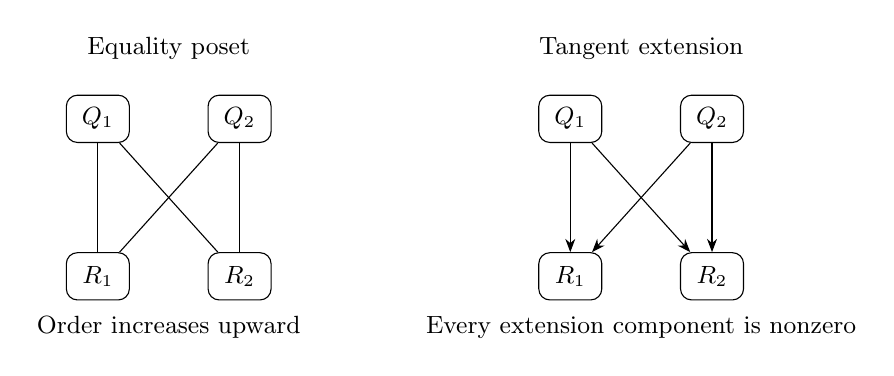
\begin{tikzpicture}[x=1cm,y=1cm,>=Stealth,
 every node/.style={font=\small},factor/.style={draw,rounded corners,
 fill=white,minimum width=8mm,minimum height=6mm}]
\begin{scope}
 \node at (0,2.9) {Equality poset};
 \node[factor] (a1) at (-.9,0) {\(R_1\)};
 \node[factor] (a2) at (.9,0) {\(R_2\)};
 \node[factor] (b1) at (-.9,2) {\(Q_1\)};
 \node[factor] (b2) at (.9,2) {\(Q_2\)};
 \foreach \i in {1,2} \foreach \j in {1,2}
   \draw (a\i)--(b\j);
 \node at (0,-.65) {Order increases upward};
\end{scope}
\begin{scope}[xshift=6cm]
 \node at (0,2.9) {Tangent extension};
 \node[factor] (c1) at (-.9,0) {\(R_1\)};
 \node[factor] (c2) at (.9,0) {\(R_2\)};
 \node[factor] (d1) at (-.9,2) {\(Q_1\)};
 \node[factor] (d2) at (.9,2) {\(Q_2\)};
 \foreach \i in {1,2} \foreach \j in {1,2}
   \draw[->] (d\j)--(c\i);
 \node at (0,-.65) {Every extension component is nonzero};
\end{scope}
\end{tikzpicture}
\caption{The crown fourfold: equality order and extension orientation.
For general \(X_k\), replace the two upper vertices by \(2k\)
vertices; every upper vertex is joined to both lower vertices.
The extension arrows point toward the subbundle factors.}
\label{fig06:poset}
\end{figure}


% ============================================================
% section_07_extension.tex
% ============================================================
\section{The actual tangent extension}\label{sec07:extension}

The relative tangent of a quotient projective bundle
\(\PP_B(\cO\oplus L)\) is \(\cO(2\xi)\otimes L^{-1}\),
as follows from the rank-two relative Euler sequence. The relative
tangent of a fibre product of smooth morphisms is the direct sum of
the pulled-back relative tangents. The base tangent is
\(\bigoplus_j\cO_B(2h_j)\). These observations prove the exact
sequence \eqref{eq01:extension}. Its factors have first Chern
classes \(C_p\), hence are pairwise nonisomorphic. As line bundles
they are stable, and their slopes at \(H_0\) are equal. Refining
the subobject by its two summands and the quotient by its \(d\)
summands gives a Jordan--H\"older filtration with locally free
graded bundle.

\begin{proposition}\label{prop07:components}
Every component of the extension \eqref{eq01:extension} in
\(\Ext^1(Q_j,R_i)\) is nonzero. It is the image of
\(\pm\epsilon_j\) times a fixed generator of
\(H^1(B,\cO_B(-2h_j))\) under the coefficient map defined by the
fibre vector field \(z_i\partial/\partial z_i\).
\end{proposition}

\begin{proof}
Trivialize \(L\) on base charts \(U_a\), with transitions \(g_{ab}\).
On an affine projective fibre chart the coordinate transforms as
\(z_{i,b}=g_{ab}^{\pm1}z_{i,a}\), with one consistent choice of sign.
Differentiating gives the off-diagonal tangent transition
\begin{equation}\label{eq07:cocycle}
 \pm d\log g_{ab}\otimes
                \left(z_i\frac{\partial}{\partial z_i}\right).
\end{equation}
The vector field extends over the other projective chart and defines
a global section of \(R_i\). The \(i\)-th row is therefore the
image of the Atiyah class of \(L\) in \(H^1(B,\Omega_B^1)\).
Since \(c_1(L)=\sum_j\epsilon_jh_j\), its \(j\)-th component
is the stated nonzero multiple before applying the coefficient map.

This map remains injective on that cohomology group. The three
fibrewise vector fields give
\begin{equation}\label{eq07:pushforward}
 \pi_*R_i=L^{-1}\oplus\cO_B\oplus L,
 \qquad R^q\pi_*R_i=0\quad(q>0).
\end{equation}
The middle summand is generated by \(z_i\partial/\partial z_i\).
On the active fibre the bundle is \(\cO_{\PP^1}(2)\); the other
fibre contributes its structure sheaf. Both have no higher
cohomology, proving the vanishing in \eqref{eq07:pushforward}.
Leray and the projection formula identify the induced map on
\(H^1\) with inclusion of the direct summand
\(\cO_B(-2h_j)\). Its one-dimensional \(H^1\) has nonzero
generator, and \(\epsilon_j=\pm1\). All \(2d\) components survive.
\end{proof}

Thus the actual extension support has arrows \(Q_j\to R_i\) for
every pair \((i,j)\). Its underlying graph is the same complete
bipartite graph as the equality poset, with the arrows reversed.
The orientation distinction is recorded in Figure~\ref{fig06:poset}.
After a smooth splitting, the off-diagonal Dolbeault entry \(\beta\)
maps \(\bigoplus Q_j\) to \(R_1\oplus R_2\) and vanishes on
the latter. Hence \(\beta\wedge\beta=0\), as for every two-step
extension of this form. Here integrability is already supplied by
the actual tangent bundle; it is not inferred merely from a drawn
graph. The graph also contains undirected cycles, so a tree-only
spectral result would not cover this example.

We next identify the equality subbundles as foliations with explicit
smooth leaf-space morphisms. Put \(Y_i=\PP_B(\cO\oplus L)\) for
the two factors, and, for \(J\subset\{1,\ldots,d\}\), put
\(B_{J^c}=\prod_{j\notin J}\PP^1\).

\begin{proposition}\label{prop07:relative}
The equality line \(\mathcal F_{\CC e_i}=R_i\) is
\(T_{X_k/Y_{3-i}}\). For the subspace \(V_J\) in
\eqref{eq06:subspaces},
\begin{equation}\label{eq07:relative}
 \mathcal F_{V_J}=T_{X_k/B_{J^c}}.
\end{equation}
All the morphisms here are smooth and projective, and these are
equalities of saturated subbundles in \(T_{X_k}\).
\end{proposition}

\begin{proof}
Projection to the other projective-bundle factor is a smooth
projective-line bundle, with relative tangent \(R_i\).
The map \(X_k\to B_{J^c}\) is the composition of the smooth
\((\PP^1)^2\)-bundle \(X_k\to B\) with the smooth base projection.
Its differential is surjective, so its kernel is a saturated
subbundle. On the dense torus its generic tangent subspace is
exactly \(V_J\). A saturated subsheaf of a vector bundle is uniquely
determined by its generic subspace: it is the intersection of that
subspace with the bundle inside its rational generic fibre.
This proves \eqref{eq07:relative} and the line assertion.
\end{proof}

Together with Sections~\ref{sec05:family}--\ref{sec06:classification}
and Proposition~\ref{prop04:dimension}, these results complete the
proof of Theorem~\ref{thm01:family}. They concern the specified
saturated equivariant equality objects. A modification supported in
codimension two can have the same slope without being a subbundle;
no assertion about all such modifications is intended.

% ============================================================
% section_08_hn.tex
% ============================================================
\section{Local Harder--Narasimhan filtrations}\label{sec08:hn}

We again allow the general toric equality data of
Section~\ref{sec02:equality}. For an ideal \(I\subset P\), write
\(r(I)=\sum_{p\in I}r_p\), \(z(I)=\sum_{p\in I}z_p\), and
\(\mathcal F_I\) for its saturated tangent subsheaf.
No local-freeness assumption is made in this section.

Harder--Narasimhan filtrations exist for torsion-free sheaves at the
real ample-power classes used here. More generally the real movable
framework gives existence, saturation, uniqueness, and strictly
decreasing semistable quotient slopes
\cite[Theorem~1.3.20 and Remarks~1.3.22--1.3.26]{pang2015}.
The unique inclusion-largest maximal destabilizer is preserved by a
connected algebraic group acting trivially on numerical classes.
Thus all HN terms here are equivariant. The finite curve-class
decompositions and quotient-preimage procedure of Neumann and Pang
\cite[Theorem~3.3.4 and Proposition~3.3.5]{neumann2009}
\cite[Proposition~2.1.19 and \S2.2]{pang2015} are prior results.
The following theorem identifies which finite objects suffice on
one common neighborhood of a semistable class.

\begin{theorem}\label{thm08:hn}
After shrinking once around \(H_0\), every ordinary HN term of
\(T_X\) is one of the original equality subsheaves \(\mathcal F_I\).
Given a current ideal \(I\), the next term is the inclusion-largest
ideal \(J\supsetneq I\) maximizing
\begin{equation}\label{eq08:greedy}
 \frac{z(J)-z(I)}{r(J)-r(I)}.
\end{equation}
The common slope \(\mu_H(T_X)\) is subtracted in this formula.
In particular the whole local HN flag decomposition is determined by
\((P,r,L_{\rm acc})\) in the coordinates of
Theorem~\ref{thm03:normal}.
\end{theorem}

\begin{proof}
We prove the finite exclusion simultaneously in all equality
intervals. Fix ideals \(I\subsetneq J\) and put
\(\mathcal Q=\mathcal F_J/\mathcal F_I\). It is torsion free and
saturated in \(T_X/\mathcal F_I\), since \(T_X/\mathcal F_J\)
is torsion free. If \(\mathcal G\subset\mathcal Q\) is saturated,
its preimage \(\widetilde{\mathcal G}\subset T_X\) is saturated:
the sequence
\begin{equation}\label{eq08:preimage}
 0\longrightarrow\mathcal Q/\mathcal G
 \longrightarrow T_X/\widetilde{\mathcal G}
 \longrightarrow T_X/\mathcal F_J\longrightarrow0
\end{equation}
has torsion-free end terms. For an equivariant \(\mathcal G\), the
preimage is torus-invariant and saturated. Klyachko's classification
\cite{klyachko1990} therefore identifies it with \(\mathcal F_W\)
for a complex subspace \(V_I\subset W\subset V_J\subset N_\CC\).
Its quotient slope is
\begin{equation}\label{eq08:quotient}
 \mu_H(\mathcal F_W/\mathcal F_I)
  =\frac{(C_W-C_I)H^{n-1}}{\dim W-r(I)},\qquad
 C_W=\sum_{v_\rho\in W}D_\rho.
\end{equation}
At \(H_0\), the whole interval \(\mathcal Q\) has slope \(\tau\)
and is semistable: a subobject of greater slope would, by its
preimage, contradict semistability of \(T_X\).

Choose the equivariant inclusion-largest subobject of maximal slope
in \(\mathcal Q\), allowing \(\mathcal Q\) itself; its existence
and equivariance follow from the real-class HN theorem above.
Its slope is positive on a small neighborhood because it is at least
\(\mu_H(\mathcal Q)\), which is close to \(\tau>0\). Replace
its preimage subspace \(W\) by
\[
 W'=\spanC\bigl(V_I,\{v_\rho:v_\rho\in W\}\bigr).
\]
The numerator in \eqref{eq08:quotient} is unchanged and
nonnegative; positivity of the slope makes it positive.
The denominator weakly decreases. A strict decrease would give a
larger slope, contradicting maximality. Thus every relevant
maximizer is in the finite list of spaces spanned by \(V_I\) and
a subset of the ray vectors, inside \(V_J\).

At \(H_0\), such a quotient has slope \(\tau\) exactly when
\(W\) is tight: add the degree \(\tau r(I)\) of \(\mathcal F_I\)
in \eqref{eq08:quotient}. Otherwise its slope is strictly smaller
than that of the whole interval. There are finitely many equality
intervals and finitely many candidates in each. Shrink once so all
whole-interval slopes stay positive and every initially smaller
candidate stays smaller than its whole interval. Then every maximum
comes from an original tight ideal between \(I\) and \(J\).
This is one neighborhood valid for every successive quotient; no
iteration-dependent shrinking is needed.

Degrees and ranks are valuations on the ideal lattice. If two
ideals containing \(I\) maximize the average, their union also
maximizes it, by the valuation identities and the maximality bound
on their intersection. The empty relative intersection contributes
zero to both identities. Taking the union of all maximizers gives
a unique inclusion-largest maximizer. The next maximal slope in
the quotient is strictly smaller: an equal or larger one would
contradict respectively inclusion maximality or slope maximality
of the previous term. Each resulting quotient is semistable by
the same finite test. The defining uniqueness characterization of
the HN filtration proves the theorem. Finally
\(C_J-C_I=(r(J)-r(I))D/n+\sum_{p\in J\setminus I}K_p\)
gives exactly \eqref{eq08:greedy}.
\end{proof}

The theorem localizes the ordinary filtration, including its quotients
when they are merely torsion free. It is stronger than retaining only
the tangent stability inequalities, but is a local refinement of the
earlier quotient algorithm, rather than a replacement for it.

\begin{proposition}\label{prop08:products}
Fix an ideal flag
\(\varnothing=I_0\subsetneq I_1\subsetneq\cdots\subsetneq I_m=P\).
Put \(S_j=I_j\setminus I_{j-1}\), with its induced poset, and
\(R_j=\sum_{p\in S_j}r_p\). Decompose uniquely
\[
 z_p=r_p\lambda_j+w_p\quad(p\in S_j),\qquad
 \sum_{p\in S_j}w_p=0.
\]
Its HN region in the full space \(Z\) is exactly
\begin{equation}\label{eq08:region}
 \lambda_1>\cdots>\lambda_m,\qquad
 \sum_jR_j\lambda_j=0,\qquad
 w|_{S_j}\in\cC(S_j)\quad(1\le j\le m).
\end{equation}
It is linearly isomorphic to
\begin{equation}\label{eq08:product}
 \RR_{>0}^{m-1}\times\prod_{j=1}^m\cC(S_j),\qquad
 \dim=|P|-1-\sum_{j=1}^m(c(S_j)-1).
\end{equation}
For actual polarizations intersect \eqref{eq08:region} with
\(L_{\rm acc}\) and add the free coordinates. If \(L_{\rm acc}=Z\),
every flag occurs arbitrarily near \(H_0\).
\end{proposition}

\begin{proof}
The interval of ideals \([I_{j-1},I_j]\) is the ideal lattice of
\(S_j\). After subtracting the segment slope, its semistability
inequalities are precisely the ideal sums of \(w|_{S_j}\).
Theorem~\ref{thm08:hn} makes these tests complete in the common
neighborhood. Strictly decreasing segment slopes are the remaining
HN requirement, proving \eqref{eq08:region}. Consecutive slope
gaps give arbitrary positive coordinates; their weighted mean-zero
condition fixes the common additive constant. Lemma~\ref{lem03:root}
gives \(\dim\cC(S_j)=|S_j|-c(S_j)\), proving the dimension.
For occurrence set \(w=0\) and choose strictly decreasing
\(\lambda_j\) with weighted mean zero. Scale toward the origin
and use the inverse ample-power coordinates.
\end{proof}

Each region is convex and contractible. It includes any semistable
boundary directions inside its individual HN quotients. In particular,
it need not be relatively open, and its closure need not be a union
of entire other HN regions. A finite central arrangement obtained by
equating ideal-interval slopes refines the description, but the
statement above is not a global HN fan theorem.

\begin{corollary}\label{cor08:counts}
For the family \(X_k\), every nearby HN term is one of the relative
tangent subbundles in Proposition~\ref{prop07:relative}. Every ideal
flag occurs. If \(F(m)\) denotes the ordered Bell number, the number
of flags is \(6F(2k)\). For \(k=1\), there are thirteen regions of
dimension three, four of dimension two, and one of dimension one
in \(Z\), before the one free polarization coordinate.
\end{corollary}

\begin{proof}
Full accessibility and the relative-tangent identification were
proved in Sections~\ref{sec06:classification}--\ref{sec07:extension}.
The count is a finite poset argument. In \(K_{a,b}\), a flag either
contains the full ideal of minima, or passes it in a unique mixed
segment. In the first case it gives independent ordered partitions
of the \(a\) minima and \(b\) maxima, counted by \(F(a)F(b)\).
In the second case splitting the mixed segment into its last
minimal block followed by its first maximal block gives the same
pair of ordered partitions. Conversely merging those two blocks
recovers exactly one flag of the second type. Thus the total is
\(2F(a)F(b)\). Since \(F(2)=3\), our family has \(6F(2k)\).

For the crown the nine flags that pass through the full ideal of
minima have four, four, and one regions in dimensions three, two,
and one. This follows by choosing either two ordered singleton
blocks or one double block on each side: a double block is an
antichain and lowers the dimension by one in
\eqref{eq08:product}. Each of the other nine flags has one mixed
connected segment and any remaining pure segments are singletons.
All nine are three-dimensional. Summing gives the stated counts.
\end{proof}

The quotients between these HN terms on \(X_k\) are locally free.
Indeed the terms are nested relative tangent subbundles, and their
generic inclusions are their inclusions as kernels of the indicated
projections; on fibres these have constant ranks. This is a feature
of this family, not a local-freeness consequence of the general
numerical normal form.

% ============================================================
% section_09_fourfold.tex
% ============================================================
\section{The fourfold and its analytic parameters}\label{sec09:fourfold}

For \(k=1\), let \(B=\PP^1\times\PP^1\) and \(L=\cO_B(1,-1)\).
The complete ray matrix, in the order of \eqref{eq05:rays}, is
\begin{equation}\label{eq09:matrix}
 \begin{pmatrix}
 1&-1&0&0&0&1&0&-1\\
 0&0&1&-1&0&1&0&-1\\
 0&0&0&0&1&-1&0&0\\
 0&0&0&0&0&0&1&-1
 \end{pmatrix}.
\end{equation}
One ray from each consecutive pair gives the sixteen maximal cones.
The exact intersections simplify to
\begin{equation}\label{eq09:values}
 \begin{gathered}
 \eta_i^2=-\tfrac12h_1h_2,\qquad F_1(r)=r^2-\tfrac16,\qquad
 G_1(r)=-2r^2+2r+\tfrac23,\\
 r_1=\frac{3+\sqrt{21}}6,\qquad H_0^4=16+4\sqrt{21},\\
 C_pH_0^3=6+2\sqrt{21},\qquad
 D_\rho H_0^3=3+\sqrt{21}.
 \end{gathered}
\end{equation}
The irrationality is a property of this reference divisor ray;
nearby stable integral polarizations still exist.
At the rational ample test classes \(r=5/4\) and \(r=3/2\),
the block degrees \((C_1H_r^3,\ldots,C_4H_r^3)\) are respectively
\[
 (59/4,59/4,15,15),\qquad (23,23,18,18).
\]
An exact check of every ray flat gives strict stability at \(5/4\),
whereas the relative tangent line \(R_1\) destabilizes at \(3/2\).
At \(r=1\) one of the base intervals in \eqref{eq05:polytope}
collapses; the class is not ample. These checks distinguish the
equal-slope construction from a merely formal solution in curve
space. The all-\(k\) statements rely on the preceding proofs.

% Native figure source: figures/code/fig09_square.tex
\begin{figure}[htbp]
\centering
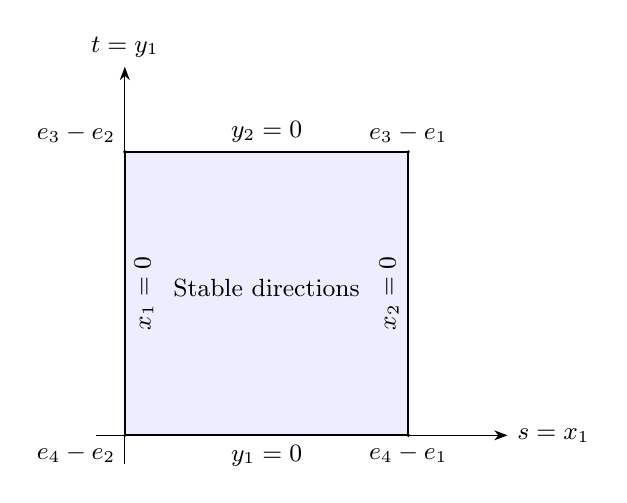
\begin{tikzpicture}[x=3.6cm,y=3.6cm,>=Stealth,
 every node/.style={font=\small}]
 \fill[blue!7] (0,0) rectangle (1,1);
 \draw[thick] (0,0) rectangle (1,1);
 \draw[->] (-.1,0)--(1.35,0) node[right] {\(s=x_1\)};
 \draw[->] (0,-.1)--(0,1.3) node[above] {\(t=y_1\)};
 \foreach \x/\y in {0/0,0/1,1/0,1/1} \fill (\x,\y) circle (.65pt);
 \node[below left] at (0,0) {\(e_4-e_2\)};
 \node[above left] at (0,1) {\(e_3-e_2\)};
 \node[below] at (1,0) {\(e_4-e_1\)};
 \node[above] at (1,1) {\(e_3-e_1\)};
 \node at (.5,.52) {Stable directions};
 \node[rotate=90,below] at (0,.5) {\(x_1=0\)};
 \node[rotate=90,above] at (1,.5) {\(x_2=0\)};
 \node[above] at (.5,1) {\(y_2=0\)};
 \node[below] at (.5,0) {\(y_1=0\)};
\end{tikzpicture}
\caption{The square section of the fourfold chamber, in coordinates
\(z=(-s,-(1-s),t,1-t)\). The four vertices represent extreme rays
and the four edges represent facets. The proper ideal consisting of
both minima has sum \(-1\) throughout this section; its equality
occurs only at the apex of the full cone.}
\label{fig09:square}
\end{figure}


The fourfold has seven tight subspaces including zero and the whole
space, with the five proper nonzero ones
\[
 \CC e_1,\quad\CC e_2,\quad
 \spanC(e_1,e_2),\quad
 \spanC(e_1,e_2,f_1),\quad\spanC(e_1,e_2,f_2).
\]
The square in Figure~\ref{fig09:square} records the four rays and
four facets of its centered chamber. The HN regions outside and on
this chamber carry the additional flag information of
Corollary~\ref{cor08:counts}; eighteen is a count of filtration
flags, not a count of full-dimensional stable chambers.

\subsection*{Parameters for the analytic application}
For every \(X_k\), order the line factors as
\((R_1,R_2,Q_1,\ldots,Q_d)\), and define
\begin{equation}\label{eq09:demands}
 \begin{aligned}
 V(H)&=H^n/n!,&
 z_v(H)&=(C_v-D/n)H^{n-1},\\
 \kappa_v(H)&=\frac{2\pi C_vH^{n-1}}{(n-1)!V(H)},&
 b_v(H)&=-\biggl(\kappa_v(H)-\frac1n\sum_w\kappa_w(H)\biggr)
       =-\frac{2\pi z_v(H)}{(n-1)!V(H)}.
 \end{aligned}
\end{equation}
The \(\kappa_v\) are the Hermitian--Einstein constants for the line
factors when the Kähler form represents \(H\). The minus sign
reverses the upward poset orientation to the extension orientation
\(Q_j\to R_i\). For stable polarizations these centered constants satisfy
\begin{equation}\label{eq09:signs}
 x_i=b_{R_i}>0,\qquad y_j=-b_{Q_j}>0,
 \qquad\sigma=x_1+x_2=\sum_jy_j.
\end{equation}
The factor ranks are all one; no rank factors are suppressed in
these equalities.

\begin{proposition}\label{prop09:chart}
There is an analytic chart \(H=H(s)\) on a full neighborhood of
\(H_0\) in its fixed-volume hypersurface, with
\begin{equation}\label{eq09:chart}
 H(0)=H_0,\qquad V(H(s))=V_0,
 \qquad b(H(s))=s\in Z,\qquad |H(s)-H_0|\le C\|s\|.
\end{equation}
On its stable part \(\|s\|_1=2\sigma\), hence
\(|H(s)-H_0|=O(\sigma)\). It admits smooth Kähler representatives
\(\omega_s\) with \(\|\omega_s-\omega_0\|_{C^a}=O_a(\|s\|)\)
for every fixed \(a\). The reference representative \(\omega_0\)
can be invariant under interchange of the two projective factors.
\end{proposition}

\begin{proof}
Full accessibility gives \(\rk dz_{H_0}=n-1\). Homogeneity and
\(z(H_0)=0\) put \(H_0\) in its kernel, which is therefore
exactly \(\RR H_0\). Moreover \(dV_{H_0}[H_0]=nV_0\ne0\).
The restriction of \(dz\) to \(\ker dV\) is an isomorphism onto
\(Z\). The derivative of the volume denominator in
\eqref{eq09:demands} contributes zero at \(z=0\), so the same
is true for \(db\). The analytic inverse-function theorem on the
fixed-volume hypersurface proves the chart and its derivative bound.
Equation~\eqref{eq09:signs} gives the \(\ell^1\) identity.

The reference class is invariant under fibre exchange. Average any
Kähler representative over this involution to choose \(\omega_0\).
Represent a basis of the real divisor space by smooth closed real
\((1,1)\)-forms, and add the linear combination corresponding to
\(H(s)-H_0\). Positivity is open, so this supplies the claimed
family and all derivative bounds after shrinking.
\end{proof}

The chart includes every sufficiently small centered constant vector,
not only those on a symmetric path. Requiring every representative to be invariant
under fibre exchange would impose equal fibre slopes and lose this
property. Only the reference form is required to be invariant.
The tangent extension, its actual nonzero components, and this full
controlled parameter chart are the geometric inputs to the analytic
companions. Neither the fan nor the chamber computes absolute
harmonic extension norms. Such coefficients, and any symmetry used to
simplify them at the reference form, belong to the metric analysis.

\subsection*{Exact checks and further questions}
The printed fan, maximal-cone rule, and ring determine all the
calculations above. Supporting exact computations use rational row
reduction to enumerate ray flats, and compare Chow-ring intersections
with \eqref{eq05:volume} independently. For \(k=1,2,3\) the counts
are shown in Table~\ref{tab09:checks}; the finite calculation is
not the proof for arbitrary \(k\).

\begin{table}[htbp]
\centering
\caption{Exact finite checks. Ray-flat and tight counts include zero
and the full space. HN flags include regions of every dimension.}
\label{tab09:checks}
\begin{tabular}{@{}rrrrrr@{}}
\toprule
\(k\)&\(n=\rho\)&Maximal cones&Ray flats&Tight flats&HN flags\\
\midrule
1&4&16&34&7&18\\
2&6&64&274&19&450\\
3&8&256&2314&67&28098\\
\bottomrule
\end{tabular}
\end{table}

The reproducible calculations also check deliberate failure cases.
The ample test fails at \(r=1\). A positive class above the wall
has an explicit destabilizing relative line. With all twists set
to zero, the ray-flat computation gives all sixteen coordinate
subspaces as tight in dimension four, an antichain rather than a
crown. The HN enumeration compares the maximal-average rule with
the independent flag inequalities \eqref{eq08:region} and records
one direction for every crown flag. Computation sources accompany
the manuscript, including the native figure descriptions.

The examples settle nonsimplicial tangent-chamber realization in
the stated smooth-projective weak-Fano class. General Fano
realizations, arbitrary equality posets, realizability of dependent
accessible sections, and global chamber gluing remain open here.
The low-dimensional restriction does not realize the diamond, and
the relative-tangent result is not a classification of all
foliations or Mori contractions. Singular graded sheaves and
higher-step extension integrability require further analysis.

% ============================================================
% section_10_obstructions.tex
% ============================================================
\section{An obstruction for positive-twist Bott towers}
\label{sec10:obstruction}

The crown construction does not realize the four-element diamond.
There is a natural iterated projective-bundle construction with the
corresponding arrangement of tangent factors, but its slope equations
already obstruct the proposed realization in a positive-twist family.

For positive integers $t,u$, let
\[
 B_t=\PP_{\PP^1}(\cO\oplus\cO(t))
       \times_{\PP^1}\PP_{\PP^1}(\cO\oplus\cO(t)),\qquad
 X_{t,u}=\PP_{B_t}\bigl(\cO\oplus\cO(u(x_1+x_2))\bigr).
\]
Write $f$ for the base point class, $x_1,x_2$ for the quotient
tautological classes on $B_t$, and $y$ for the last tautological
class. Pullbacks are implicit. The relative tangent sequences are
\[
 0\to\cO(C_3)\to T_X\to\pi^*T_{B_t}\to0,\qquad
 0\to\cO(C_1)\oplus\cO(C_2)\to T_{B_t}\to\cO(C_0)\to0,
\]
where
\[
 C_0=2f,\quad C_1=2x_1-tf,\quad C_2=2x_2-tf,\quad
 C_3=2y-u(x_1+x_2).
\]
Inverse images of the two middle line summands give the natural
diamond-shaped arrangement. This description does not assert that
it is an equal-slope arrangement, or identify all extension components.

\begin{proposition}\label{prop10:bott}
For every $t,u\ge1$, no ample real class on $X_{t,u}$ makes all four
natural tangent line factors have equal slope.
\end{proposition}

\begin{proof}
The projective-bundle intersection ring satisfies
\[
 f^2=0,\quad x_i^2=tf x_i,\quad
 y^2=u(x_1+x_2)y,\quad \int_Xfx_1x_2y=1.
\]
Every numerical divisor class has a unique expression
$H=af+bx_1+cx_2+dy$, and it is ample exactly when $a,b,c,d>0$.
To verify this cone, observe that for a nef line bundle $L$ the nef
cone of $\PP(\cO\oplus L)$ consists of $q\xi+\pi^*A$ with
$q\ge0$ and $A$ nef. Necessity follows from a fibre and the section
of the quotient $\cO$, and sufficiency from nefness of $\xi$.
Apply this successively, since every twist here is nef, and take
the interior. These are standard split projective-bundle calculations;
compare \cite[\S2 and Corollary~3.1.2]{khandasgupta2019}.

For arbitrary ample $H$, the ring gives
\begin{equation}\label{eq10:middle}
 (C_1-C_2)H^3=6d(c-b)\bigl(t(b+c+ud)+2a\bigr).
\end{equation}
The factor in parentheses is positive, so equality forces $b=c$.
Put $S=x_1+x_2$. For this forced value, push down to $B_t$:
\[
 \pi_*H^3=MfS+NS^2,\quad
 M=3ad(2b+ud),\quad N=d(3b^2+3bud+u^2d^2).
\]
The products $\int_B fS^2=2$, $\int_Bx_1fS=1$ and
$\int_Bx_1S^2=3t$ then give
\begin{equation}\label{eq10:base}
 (C_0-C_1)H^3=-4(t-1)N-2M<0,
\end{equation}
contradicting equal slopes. For an explicit derivation of
\eqref{eq10:middle}, write $A=af+bx_1+cx_2$ and $L=uS$.
The integrals against $x_1-x_2$ of $A^2,AL,L^2$ are respectively
$(c-b)(t(b+c)+2a)$, $ut(c-b)$ and $0$; apply
$\pi_*H^3=3dA^2+3d^2AL+d^3L^2$ and multiply by two.
\end{proof}

The proposition excludes the natural filtration construction throughout
this family. It does not exclude every equality poset on these
fourfolds, arbitrary signed Bott towers, or diamond realizations in
general. Nor does it assert instability at every polarization.
These fourfolds are not Fano: the $f$ coefficient of
\[
 -K_X=(2-2t)f+(2-u)(x_1+x_2)+2y
\]
is nonpositive in the ample cone just computed.

% ============================================================
% section_11_cy.tex
% ============================================================
\appendix
\section{The fourfold, toric contractions, and a Calabi--Yau transition}
\label{sec11:cy}

The fourfold of Section~\ref{sec09:fourfold} also permits an explicit
comparison with anticanonical Calabi--Yau hypersurfaces. This comparison
does not identify tangent stability walls with toric birational walls.
It exhibits different tangent stability within one toric chamber while
the hypersurface and its deformation problem remain fixed.

Let $B=\PP^1\times\PP^1$, $L=\cO_B(1,-1)$, and
\[
 X=\PP_B(\cO\oplus L)\times_B\PP_B(\cO\oplus L).
\]
Write $f,g$ for the base hyperplane classes, $\xi_1,\xi_2$ for the
quotient tautological classes, and $\eta_i=\xi_i-(f-g)/2$. Then
\[
 H_r=\eta_1+\eta_2+r(f+g),\qquad r>1,\qquad -K_X=2H_1.
\]

\begin{proposition}\label{prop11:transition}
The tangent bundle is stable at $H_{5/4}$ and unstable at $H_{3/2}$,
although both classes lie in one chamber of the toric divisor-class
GKZ decomposition. The anticanonical model of $X$ has two disjoint
singular projective lines, each transversely an ordinary threefold node.
A general anticanonical hypersurface $Y_0$ has eight ordinary double
points and a projective small crepant resolution $Y\subset X$ with
Hodge numbers $(h^{1,1},h^{2,1})=(4,60)$. The exceptional curve classes
have rank two in $H_2(Y,\mathbb Q)$ and a six-dimensional relation
space. The threefold $Y_0$ admits a smoothing with Hodge numbers
$(2,66)$.
\end{proposition}

\begin{proof}
Number the rays, in order, as
\begin{equation}\label{eq11:rays}
 e_1,-e_1,e_2,-e_2,f_0,e_1+e_2-f_0,g_0,-e_1-e_2-g_0.
\end{equation}
The fan chooses one ray from each pair, giving sixteen unimodular
maximal cones. For $H_r$, the four fibre-ray divisor degrees equal
$A=6r^2-2$ and the four base-ray degrees equal $B=6r$; the tangent
slope is $A+B$. There are $6,15,11$ proper ray flats of ranks
$1,2,3$. Their largest unnormalized margins
$\sum_{v_\rho\in V}D_\rho H_r^3-(\dim V)(A+B)$ at the two
test points are
\[
\begin{array}{c|ccc}
r&A&B&\text{largest margin}\\\hline
5/4&59/8&15/2&-1/8\\
3/2&23/2&9&5.
\end{array}
\]
These are obtained by taking the linear closures of all ray subsets;
the complete rational lists accompany the paper. In particular all
tests are strict at $5/4$, while a fibre line already destabilizes at
$3/2$. Both classes are ample by the support inequalities of
Section~\ref{sec05:family}. The interior of this ample cone is one
GKZ chamber for the fixed fan rays, with support numbers considered
modulo principal linear functions. It is not a secondary fan for a
different configuration of hypersurface monomials. The two decompositions
therefore differ; the tangent wall is the interior class
$r=(3+\sqrt{21})/6$.

For the anticanonical contraction use the polar sign convention
\[
 \Delta=\{m:\langle m,v_i\rangle\le1\},\qquad Q=\operatorname{conv}(v_i).
\]
In dual coordinates $(x,y,z,w)$ its inequalities are
\begin{equation}\label{eq11:polar}
 -1\le x,y\le1,\qquad x+y-1\le z\le1,\qquad
 -x-y-1\le w\le1.
\end{equation}
It has twelve integral vertices. The sixteen cones refine its normal
fan. The only nonsimplicial maximal cones contain one of the circuits
\begin{equation}\label{eq11:circuits}
 \tau_f=\{0,2,4,5\},\quad v_0+v_2=v_4+v_5,
 \qquad
 \tau_g=\{1,3,6,7\},\quad v_1+v_3=v_6+v_7,
\end{equation}
and one ray of the remaining base pair. For $\tau_f$ the first three
rays form a basis of its saturated rank-three lattice and the fourth
is $(1,1,-1)$ in that basis; adjoining either remaining base ray is
a lattice basis in dimension four. The same statement holds for
$\tau_g$. Thus the four nonsimplicial affine charts are ordinary
conifold charts times an affine line, with no finite lattice quotient.
All other maximal cones are unimodular. The transverse quotient fan
of each circuit has two opposite primitive rays, giving a singular
$\PP^1$. The two curves are disjoint: a cone containing both circuits
would contain $e_1$ and $-e_1$.

Their dual edges in $\Delta$ are
\[
 [(1,1,1,-3),(1,1,1,1)],\qquad
 [(-1,-1,-3,1),(-1,-1,1,1)].
\]
Both have lattice length four, so the descended anticanonical bundle
restricts to $\cO(4)$ on each singular line. All five edge monomials
occur. A general section has four simple zeros on each line, away
from the fixed endpoints. Near such a zero its derivative along the
line is nonzero; eliminating that coordinate leaves the ordinary
threefold node. Bertini excludes other singularities. The toric
refinement has no new rays and is small and crepant; its restriction
gives the projective small resolution $Y\to Y_0$ with eight disjoint
exceptional curves.

Choose the section simultaneously general and $\Delta$-regular.
The fan is a smooth projective crepant subdivision using every boundary
lattice point of $Q$, hence a maximal projective crepant partial
(MPCP) subdivision in the terminology
of \cite{batyrev1994}. Direct enumeration in \eqref{eq11:polar} gives
\[
 l(\Delta)=69,\quad l(Q)=9,\qquad
 \begin{array}{c|rrrrr}
 \text{codimension of the relative interior}&0&1&2&3&4\\\hline
 \Delta&1&4&22&30&12\\
 Q&1&0&0&0&8.
 \end{array}
\]
Here the table counts lattice points, not faces. Every dual edge
contributing to the codimension-two correction is primitive.
Batyrev's formula \cite[Corollary~4.5.1]{batyrev1994} therefore gives
$h^{1,1}(Y)=9-5=4$ and $h^{2,1}(Y)=69-5-4=60$.
Adjunction gives $K_Y\simeq\cO_Y$. The sequence
$0\to K_X\to\cO_X\to\cO_Y\to0$, toric structure-sheaf vanishing
and Serre duality give connectedness and
$H^1(\cO_Y)=H^2(\cO_Y)=0$.

In the divisor basis $(f,g,\xi_1,\xi_2)$ the two contracted ambient
curve classes have pairing vectors
\[
 \Gamma_f=(1,0,0,0),\qquad \Gamma_g=(0,1,-1,-1),
\]
by \eqref{eq11:circuits}. To identify their classes on $Y$, put
$D=-K_X$. The intersection ring
$f^2=g^2=0$, $\xi_i^2=(f-g)\xi_i$ and
$\int_Xfg\xi_1\xi_2=1$ gives
\begin{equation}\label{eq11:gram}
 \left(\int_X D_iD_jD^2\right)_{i,j}
 =\begin{pmatrix}
 0&8&4&4\\8&0&12&12\\4&12&-8&0\\4&12&0&-8
 \end{pmatrix},\qquad \det=-16384.
\end{equation}
Thus the four divisor restrictions are independent on $Y$ and span
$H^2(Y,\mathbb Q)$, since $h^{1,1}(Y)=4$ and $H^{2,0}(Y)=0$.
Their pairings determine rational homology classes. The four curves
over each singular line have the same class in $H_2(Y,\mathbb Q)$,
and the two types are independent. The full relation space is therefore
\begin{equation}\label{eq11:relations}
 \sum_{i=1}^4a_i=0,\qquad \sum_{i=1}^4b_i=0.
\end{equation}
In particular $(1,1,1,-3;1,1,1,-3)$ is a relation with every
coefficient nonzero. No integral saturation assertion is required.

The threefold $Y_0$ is connected, normal and projective, has trivial
dualizing bundle by Cartier anticanonical adjunction, and has only
terminal ordinary double points. Rational singularities transfer
$H^1(\cO_Y)=0$ to $Y_0$. Namikawa's smoothing criterion
\cite[Theorem~2.5]{namikawa2002} applies to the displayed relation
in $H_2(Y,\CC)$ and integrates it to a flat smoothing. With eight
nodes and exceptional rank two, conifold surgery gives
$b_2(Y_t)=4-2=2$ and $b_3(Y_t)=122+2(8-2)=134$, hence Hodge
numbers $(2,66)$.
\end{proof}

The smoothing in the proposition is an abstract deformation of $Y_0$.
It generally leaves the fixed toric hypersurface family, whose general
members still meet the two singular lines four times each. Holding
$Y_0$ fixed while varying $H_r$ changes tangent stability without
changing this relation space. The equality-poset square relation, the
two toric contraction circuits and the six-dimensional CY relation
space are distinct objects. The example supplies no canonical
identification among them and asserts no new general smoothing criterion.

The accompanying calculations enumerate all rational polar vertices,
bounded lattice points and proper ray flats, and evaluate the stated
intersections. The smoothing conclusion uses the quoted geometric
theorem, not merely the node count or finite computations.

% ============================================================
% BIBLIOGRAPHY
% ============================================================
\begin{thebibliography}{BFLR12}
\bibitem[Bat94]{batyrev1994} V.~V.~Batyrev, \emph{Dual polyhedra and mirror symmetry for Calabi--Yau hypersurfaces in toric varieties}, J. Algebraic Geom. \textbf{3} (1994), no.~3, 493--535. \href{https://arxiv.org/abs/alg-geom/9310003}{arXiv:alg-geom/9310003}.

\bibitem[BFLR12]{boussicaultferaylascouxreiner2012} A.~Boussicault, V.~F\'eray, A.~Lascoux, and V.~Reiner, \emph{Linear extension sums as valuations on cones}, J. Algebraic Combin. \textbf{35} (2012), no.~4, 573--610. \href{https://doi.org/10.1007/s10801-011-0316-2}{doi:10.1007/s10801-011-0316-2}; arXiv:1008.3278v2.

\bibitem[GRT16]{grebrosstoma2016} D.~Greb, J.~Ross, and M.~Toma, \emph{Variation of Gieseker moduli spaces via quiver GIT}, Geom. Topol. \textbf{20} (2016), no.~3, 1539--1610. \href{https://doi.org/10.2140/gt.2016.20.1539}{doi:10.2140/gt.2016.20.1539}; arXiv:1409.7564v2.

\bibitem[HNS22]{heringnillsuess2022} M.~Hering, B.~Nill, and H.~S\"u\ss, \emph{Stability of tangent bundles on smooth toric Picard-rank-2 varieties and surfaces}, in P.~Aluffi, D.~Anderson, M.~Hering, M.~Musta\c{t}\u{a}, and S.~Payne (eds.), \emph{Facets of Algebraic Geometry}, Vol.~II, London Math. Soc. Lecture Note Ser., vol.~473, Cambridge University Press, 2022, pp.~1--25. \href{https://doi.org/10.1017/9781108877855.001}{doi:10.1017/9781108877855.001}; arXiv:1910.08848v1.

\bibitem[KD19]{khandasgupta2019} B.~Khan and J.~Dasgupta, \emph{Toric vector bundles on Bott tower}, Bull. Sci. Math. \textbf{155} (2019), 74--91. \href{https://doi.org/10.1016/j.bulsci.2019.04.003}{doi:10.1016/j.bulsci.2019.04.003}; arXiv:1802.08803v2.

\bibitem[Kly90]{klyachko1990} A.~A.~Klyachko, \emph{Equivariant bundles on toral varieties}, Math. USSR-Izv. \textbf{35} (1990), no.~2, 337--375. \href{https://doi.org/10.1070/IM1990v035n02ABEH000707}{doi:10.1070/IM1990v035n02ABEH000707}.

\bibitem[Nam02]{namikawa2002} Y.~Namikawa, \emph{Stratified local moduli of Calabi--Yau threefolds}, Topology \textbf{41} (2002), no.~6, 1219--1237. \href{https://doi.org/10.1016/S0040-9383(01)00038-6}{doi:10.1016/S0040-9383(01)00038-6}.

\bibitem[Neu09]{neumann2009} S.~Neumann, \emph{A decomposition of the Moving cone of a projective manifold according to the Harder--Narasimhan filtration of the tangent bundle}, Ph.D. thesis, Albert-Ludwigs-Universit\"at Freiburg im Breisgau, November 2009. \url{https://freidok.uni-freiburg.de/data/7287}.

\bibitem[Pan15]{pang2015} T.-S.~Pang, \emph{The Harder--Narasimhan Filtrations and Rational Contractions}, Ph.D. thesis, Albert-Ludwigs-Universit\"at Freiburg im Breisgau, 2015. \href{https://doi.org/10.6094/UNIFR/10375}{doi:10.6094/UNIFR/10375}.

\bibitem[Wue26]{wuebben2026toricchambers} B.~J.~Wuebben, \emph{Local stability chambers for toric tangent bundles}, preprint, 26 October 2026, revised 27 October 2026, version~2, 17~pp. \href{https://doi.org/10.5281/zenodo.23682140}{doi:10.5281/zenodo.23682140}.
\end{thebibliography}

\bigskip
\noindent{\sc Bernd Johannes Wuebben, New York, NY,} \texttt{wuebben@gmail.com}

\end{document}
